%% LyX 1.6.7 created this file.  For more info, see http://www.lyx.org/.
%% Do not edit unless you really know what you are doing.
\documentclass[english]{article}
\usepackage{ae,aecompl}
\usepackage[T1]{fontenc}
\usepackage[latin9]{inputenc}
\usepackage[letterpaper]{geometry}
\geometry{verbose,tmargin=2.5cm,bmargin=2.5cm,lmargin=2.5cm,rmargin=2.5cm}
\usepackage{babel}

\usepackage{textcomp}
\usepackage{amsbsy}
\usepackage{graphicx}
\usepackage[numbers]{natbib}
\usepackage[unicode=true, 
 bookmarks=true,bookmarksnumbered=false,bookmarksopen=false,
 breaklinks=false,pdfborder={0 0 1},backref=false,colorlinks=false]
 {hyperref}
\hypersetup{pdftitle={Getting started with CHNOSZ},
 pdfauthor={Jeffrey M. Dick}}

\makeatletter
%%%%%%%%%%%%%%%%%%%%%%%%%%%%%% Textclass specific LaTeX commands.
\usepackage{Sweave}
\newenvironment{wrapsweave}{\par}{\par}
\newenvironment{lyxcode}
{\par\begin{list}{}{
\setlength{\rightmargin}{\leftmargin}
\setlength{\listparindent}{0pt}% needed for AMS classes
\raggedright
\setlength{\itemsep}{0pt}
\setlength{\parsep}{0pt}
\normalfont\ttfamily}%
 \item[]}
{\end{list}}

%%%%%%%%%%%%%%%%%%%%%%%%%%%%%% User specified LaTeX commands.
%\VignetteIndexEntry{1. Getting started with CHNOSZ}

\makeatother

\begin{document}

\title{Getting started with CHNOSZ}


\author{Jeffrey M. Dick}
\maketitle
\begin{wrapsweave}
\end{wrapsweave}

\section{Introduction}

This document will orient you to the basic functionality of \href{http://www.chnosz.net}{CHNOSZ},
a package for the R software environment. R is a powerful language
and also very fun to use. Don't worry if you're new to it; just plow
through the examples below and you'll start to get the hang of it.
If you want a more structured approach to learning the language, there
are some excellent guides in the Manuals section of the \href{http://www.r-project.org}{R Project page}.
You may also want to refer to a publication on CHNOSZ itself \citep{Dic08}.

The package was developed starting in 2003 to support a research project
on the thermodynamic properties of proteins. Since that time, the
functions in the package have expanded to include calculation of the
thermodynamic properties of reactions, and especially the construction
of chemical activity diagrams for both inorganic and organic systems.
The development of the package since 2009 has focused on the calculation
of the metastable equilibrium relative abundances of large numbers
of proteins with applications in interpretation of metagenomic data
and protein expression profiles.

Although I use the package primarily to model the relative stabilities
of proteins in cells and in hydrothermal systems, the database and
functions are flexible in their use. As you will see below, examples
taken from low-temperature geochemistry are used to demonstrate, and
indeed test, the package.


\section{Outline of workflow}

CHNOSZ is made up of a set of functions and supporting datasets. The
major components of the package are shown in the figure below, which
is a modified version of the flowchart shown in Ref. \citep{Dic08}
(boxes -- functions; ellipses -- datasets).

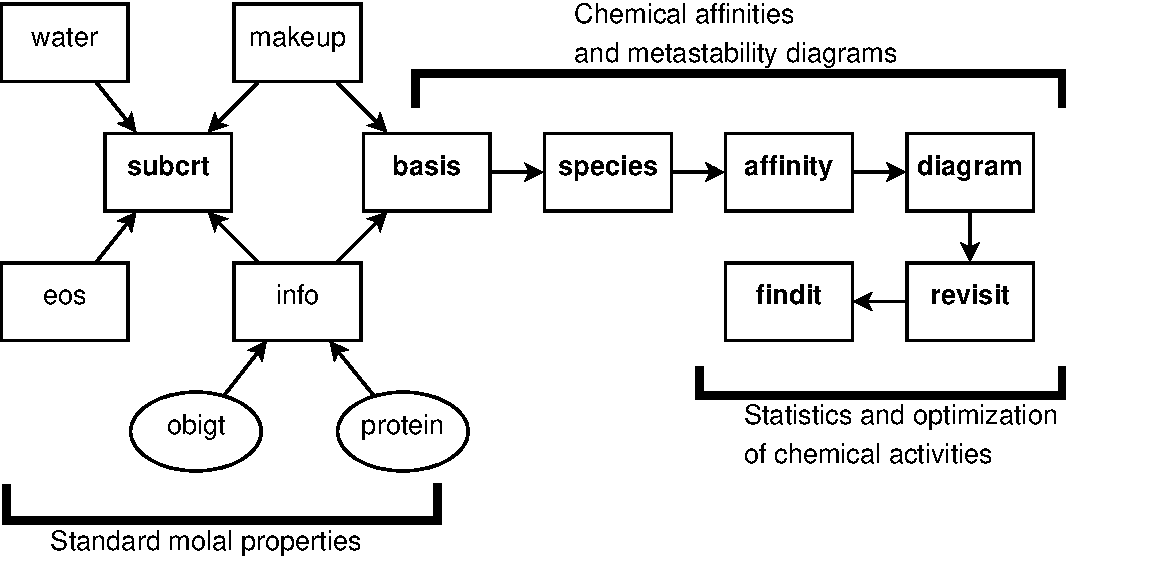
\includegraphics[width=0.8\columnwidth]{chnosz_new}

Some common usage scenarios are:
\begin{itemize}
\item using \texttt{info()} to search for species in the thermodynamic database
\item using \texttt{subcrt()} to calculate the thermodynamic properties
of species and reactions
\item using the sequence \texttt{basis()}, \texttt{species()}, \texttt{affinity()},
\texttt{diagram()} to assign the basis species that define the dimensions
of chemical composition in a system, define the species of interest
for relative stability calculations, calculate the affinities of formation
reactions of the species of interest under reference (non-equilibrium)
conditions, and to transform the non-equilibrium affinities to equilibrium
chemical activities and plot the results.
\item using \texttt{revisit()} to calculate/plot statistics of the chemical
activities of the species of interest and \texttt{findit()} to search
for combinations of activities of basis species, temperature and/or
pressure that optimize those statistics. (These features, appearing
in version 0.9-3 of the package, are not covered in this document.)
\end{itemize}
The functions are designed with an interactive setting in mind; you
can make good use of CHNOSZ without having to write your own scripts.
The examples in this vignette are meant to portray a simple interactive
session. However, as you become more familiar with CHNOSZ and R, you
will probably find it helpful to save sequences of function calls
that produce interesting results. The results can then be reproduced
on demand by yourself or others with whom you might share your scripts.


\section{Installing and loading CHNOSZ}

If you have just installed R, and you are online, installing the CHNOSZ
package should be as simple as selecting {}``Install packages from
CRAN'' or similar menu item in the R GUI or using the following command
to start the package installation process. (If you are not online,
you instead have to tell R to install the package from a local package
file.)
\begin{wrapsweave}
\begin{Schunk}
\begin{Sinput}
> install.packages("CHNOSZ")
\end{Sinput}
\end{Schunk}
\end{wrapsweave}
Then load the CHNOSZ package to make its functions and data available
in your working session.
\begin{wrapsweave}
\begin{Schunk}
\begin{Sinput}
> library(CHNOSZ)
\end{Sinput}
\end{Schunk}

\end{wrapsweave}
The rest of this document assumes that the CHNOSZ package is loaded.


\section{Thermodynamic database}


\subsection{\texttt{info()} part I}

So you want to know what are the standard molal thermodynamic properties
and equations of state parameters of aqueous ethylene? Look no further
than the \texttt{info()} function, which provides a convenient interface
to retrieve entries from the thermodynamic database packaged with
CHNOSZ.
\begin{wrapsweave}
\begin{Schunk}
\begin{Sinput}
> info("ethylene")
\end{Sinput}
\begin{Soutput}
info: ethylene (C2H4) available in aq, gas.
info: 88 refers to ethylene, C2H4 aq (SH90, 4.Sep.87)
\end{Soutput}
\end{Schunk}
\end{wrapsweave}
There are two species named {}``ethylene'' in the database. Normally,
\texttt{info()} gives preference to aqueous species if they exist,
so in this case we find that aqueous ethylene is species number 88
in the database. Let's display this entry, now by giving the numeric
value to the function.
\begin{wrapsweave}
\begin{Schunk}
\begin{Sinput}
> info(88)
\end{Sinput}
\begin{Soutput}
       name abbrv formula state source1 source2     date     G    H    S   Cp    V     a1
88 ethylene  <NA>    C2H4    aq    SH90    <NA> 4.Sep.87 19450 8570 28.7 62.5 45.5 0.7856
        a2      a3     a4   c1    c2  omega Z
88 1263.91 -1.8737 -33014 39.1 97000 -40000 0
\end{Soutput}
\end{Schunk}
\end{wrapsweave}
If you were instead interested in the properties of the gas, you could
run:
\begin{wrapsweave}
\begin{Schunk}
\begin{Sinput}
> info("ethylene", "gas")
\end{Sinput}
\begin{Soutput}
info: 2585 refers to ethylene, C2H4 gas (Sho93, 22.Sep.93)
\end{Soutput}
\end{Schunk}
\end{wrapsweave}
\texttt{info()} itself is used by other functions in the package.
It prints output to the screen, but also returns a numeric value if
it finds a species matching the search term. So, we can retrieve the
properties of aqueous acetic acid without having to futz with the
species ID number.
\begin{wrapsweave}
\begin{Schunk}
\begin{Sinput}
> aadata <- info(info("acetic acid"))
\end{Sinput}
\begin{Soutput}
info: acetic acid (C2H4O2) available in aq, liq.
info: 515 refers to acetic acid, C2H4O2 aq (Sho95, 6.Mar.92)
\end{Soutput}
\begin{Sinput}
> print(aadata)
\end{Sinput}
\begin{Soutput}
           name abbrv formula state source1 source2     date      G       H    S    Cp
515 acetic acid  <NA>  C2H4O2    aq   Sho95    <NA> 6.Mar.92 -94760 -116100 42.7 40.56
        V      a1    a2     a3     a4     c1     c2  omega Z
515 52.01 1.16198 521.8 2.5088 -29946 42.076 -15417 -15000 0
\end{Soutput}
\end{Schunk}
\end{wrapsweave}



\subsection{\texttt{thermo\$source}}

All the thermodynamic and other data, as well as system definitions
provided by the user in an interactive session, are stored in an object
called \texttt{thermo}.
\begin{wrapsweave}
\begin{Schunk}
\begin{Sinput}
> summary(thermo)
\end{Sinput}
\begin{Soutput}
         Length Class      Mode
opt      14     -none-     list
element   6     data.frame list
obigt    20     data.frame list
source    2     data.frame list
buffer    4     data.frame list
protein  25     data.frame list
stress   65     data.frame list
groups   22     data.frame list
water     0     -none-     NULL
water2    3     -none-     list
ECO      25     data.frame list
SGD      22     data.frame list
HUM      25     data.frame list
yeastgfp 28     data.frame list
basis     9     data.frame list
species  10     data.frame list
Psat      2     -none-     list
\end{Soutput}
\end{Schunk}
\end{wrapsweave}
The thermodynamic database is stored in a dataframe (an R object that
is basically a two-dimensional matrix with named columns) called \texttt{thermo\$obigt},
and the literature sources of thermodynamic data are listed in \texttt{thermo\$source}.
Most (all?) of the authors who are responsible for these data would
be highly grateful if you cite them whenever these data are used in
publications.
\begin{wrapsweave}
\begin{Schunk}
\begin{Sinput}
> ts <- thermo$source
> ts[ts$source == aadata$source1, ]
\end{Sinput}
\begin{Soutput}
   source                           reference
94  Sho95 E. L. Shock, AJS 295, 496-580, 1995
\end{Soutput}
\end{Schunk}
\end{wrapsweave}



\subsection{\texttt{info()} part II}

Want to know what acids are in the database?
\begin{wrapsweave}
\begin{Schunk}
\begin{Sinput}
> info("acid")
\end{Sinput}
\begin{Soutput}
info: no match for acid.
info: similar species names, abbreviations, or formulas are:
 [1] "a-aminobutyric acid"     "formic acid"             "acetic acid"            
 [4] "propanoic acid"          "n-butanoic acid"         "n-pentanoic acid"       
 [7] "n-hexanoic acid"         "n-heptanoic acid"        "n-octanoic acid"        
[10] "n-nonanoic acid"         "n-decanoic acid"         "n-undecanoic acid"      
[13] "n-dodecanoic acid"       "n-benzoic acid"          "o-toluic acid"          
[16] "m-toluic acid"           "p-toluic acid"           "oxalic acid"            
[19] "malonic acid"            "succinic acid"           "glutaric acid"          
[22] "adipic acid"             "pimelic acid"            "suberic acid"           
[25] "azelaic acid"            "sebacic acid"            "glycolic acid"          
[28] "lactic acid"             "2-hydroxybutanoic acid"  "2-hydroxypentanoic acid"
[31] "2-hydroxyhexanoic acid"  "2-hydroxyheptanoic acid" "2-hydroxyoctanoic acid" 
[34] "2-hydroxynonanoic acid"  "2-hydroxydecanoic acid"  "aspartic acid"          
[37] "glutamic acid"           "uracil"                  "citric acid"            
[40] "metacinnabar"            "sanidine,high"           "phosphoric acid"        
[43] "acetamide"               "nicotinamide,red"        "nicotinamide,ox"        
[46] "n-tridecanoic acid"      "n-tetradecanoic acid"    "n-pentadecanoic acid"   
[49] "n-hexadecanoic acid"     "n-heptadecanoic acid"    "n-octadecanoic acid"    
[52] "n-nonadecanoic acid"     "n-eicosanoic acid"       "hydrofluoric acid"      
[55] "NicotinamideRed"         "NicotinamideOx"         
\end{Soutput}
\end{Schunk}
\end{wrapsweave}
That's right, if \texttt{info()} can't find an exact match to a name,
it does a fuzzy search. That's why {}``uracil'' and {}``metacinnabar''
show up above. If you really just want species whose names include
the term {}``acid'', you can add a placeholder character to narrow
the search. (Note: don't use an underscore ({}``\_'') here because
that character is reserved for names of proteins. Any other character
will do; here we use a space.)
\begin{wrapsweave}
\begin{Schunk}
\begin{Sinput}
> info(" acid")
\end{Sinput}
\begin{Soutput}
info: no match for  acid.
info: similar species names, abbreviations, or formulas are:
 [1] "a-aminobutyric acid"     "formic acid"             "acetic acid"            
 [4] "propanoic acid"          "n-butanoic acid"         "n-pentanoic acid"       
 [7] "n-hexanoic acid"         "n-heptanoic acid"        "n-octanoic acid"        
[10] "n-nonanoic acid"         "n-decanoic acid"         "n-undecanoic acid"      
[13] "n-dodecanoic acid"       "n-benzoic acid"          "o-toluic acid"          
[16] "m-toluic acid"           "p-toluic acid"           "oxalic acid"            
[19] "malonic acid"            "succinic acid"           "glutaric acid"          
[22] "adipic acid"             "pimelic acid"            "suberic acid"           
[25] "azelaic acid"            "sebacic acid"            "glycolic acid"          
[28] "lactic acid"             "2-hydroxybutanoic acid"  "2-hydroxypentanoic acid"
[31] "2-hydroxyhexanoic acid"  "2-hydroxyheptanoic acid" "2-hydroxyoctanoic acid" 
[34] "2-hydroxynonanoic acid"  "2-hydroxydecanoic acid"  "aspartic acid"          
[37] "glutamic acid"           "citric acid"             "phosphoric acid"        
[40] "n-tridecanoic acid"      "n-tetradecanoic acid"    "n-pentadecanoic acid"   
[43] "n-hexadecanoic acid"     "n-heptadecanoic acid"    "n-octadecanoic acid"    
[46] "n-nonadecanoic acid"     "n-eicosanoic acid"       "hydrofluoric acid"      
\end{Soutput}
\end{Schunk}
\end{wrapsweave}
The names of species other than proteins use (almost) exclusively
lowercase letters. \texttt{info()} can also be used to search the
text of the chemical formulas as they are entered in the database;
the symbols for the elements always start with a capital letter. The
example below lists the formulas of aqueous species, then minerals,
that contain the symbol commonly used to represent the hydroxide group.
\begin{wrapsweave}
\begin{Schunk}
\begin{Sinput}
> info("(OH)")
\end{Sinput}
\begin{Soutput}
info: no match for (OH).
info: similar species names, abbreviations, or formulas are:
 [1] "B(OH)3"                       "U(OH)+3"                     
 [3] "Ti(OH)4"                      "Pd(OH)2"                     
 [5] "U(OH)+2"                      "Ru(OH)+"                     
 [7] "Ru(OH)+2"                     "Rh(OH)+"                     
 [9] "Rh(OH)+2"                     "Pd(OH)+"                     
[11] "Pt(OH)+"                      "KAl3(OH)6(SO4)2"             
[13] "Mg4Al2(Al2Si2)O10(OH)8"       "Mg2Al(AlSi)O5(OH)4"          
[15] "KFe3(AlSi3)O10(OH)2"          "Mg7Si8O22(OH)2"              
[17] "Mg48Si34O85(OH)62"            "Mg2(OH)2(CO3)*3H2O"          
[19] "Cu3(OH)2(CO3)2"               "AlO(OH)"                     
[21] "Mg(OH)2"                      "K(MgAl)Si4O10(OH)2"          
[23] "FeAl2SiO5(OH)2"               "Mg3Si2O5(OH)4"               
[25] "Mg5Al(AlSi3)O10(OH)8"         "Ca2Al3Si3O12(OH)"            
[27] "Fe2Fe(FeSi)O5(OH)4"           "Fe5Al(AlSi3)O10(OH)8"        
[29] "Al2Si2O5(OH)4"                "Na(Ca2Mg5)(AlSi7)O22(OH2)"   
[31] "Ca2FeAl2Si3O12(OH)"           "Na(Ca2Fe5)(AlSi7)O22(OH)2"   
[33] "(Fe5Al2)(Al2Si6)O22(OH)2"     "Na(Ca2Fe4Al)(Al2Si6)O22(OH)2"
[35] "(Ca2Fe5)Si8O22(OH)2"          "Al(OH)3"                     
[37] "Na2(Mg3Al2)Si8O22(OH)2"       "Fe3Si2O5(OH)4"               
[39] "Fe7Si8O22(OH)2"               "Na(Ca2Fe4Fe)(Al2Si6)O22(OH)2"
[41] "Mg5(OH)2(CO3)4*4H2O"          "CaAl2Si2O7(OH)2*H2O"         
[43] "Na(Ca2Mg4Fe)(Al2Si6)O22(OH)2" "Na2(Mg3Fe2)Si8O22(OH)2"      
[45] "Cu2(OH)2(CO3)"                "CaAl2(Al2Si2)O10(OH)2"       
[47] "Fe3Si4O10(OH)2"               "KAl2(AlSi3)O10(OH)2"         
[49] "NaAl2(AlSi3)O10(OH)2"         "Na(Ca2Mg4Al)(Al2Si6)O22(OH)2"
[51] "KFe3(AlSi3)O10(OH)O-"         "KMg3(AlSi3)O10(OH)2"         
[53] "Ca2Al2Si3O10(OH)2"            "Al2Si4O10(OH)2"              
[55] "Na2(CaMg5)Si8O22(OH)2"        "Na2(Fe3Fe2)Si8O22(OH)2"      
[57] "Mg4Si6O15(OH)2(H2O)2*4H2O"    "Fe2Al9Si4O23(OH)"            
[59] "Mg3Si4O10(OH)2"               "(Ca2Mg5)Si8O22(OH)2"         
[61] "C2H4(OH)2"                    "C3H5(OH)3"                   
\end{Soutput}
\end{Schunk}
\end{wrapsweave}



\section{Proteins}


\subsection{\texttt{protein()}}

There are few things more fun than calculating the standard molal
Gibbs energy of formation from the elements at 25 $^{\circ}$C and
1 bar of a protein using group additivity. And there are few proteins
whose thermodynamic properties more well studied than lysozyme from
the egg of the chicken.
\begin{wrapsweave}
\begin{Schunk}
\begin{Sinput}
> protein("LYSC_CHICK")
\end{Sinput}
\begin{Soutput}
  protein organism source  abbrv chains Ala Cys Asp Glu Phe Gly His Ile Lys Leu Met Asn
6    LYSC    CHICK BBA+03 P00698      1  12   8   7   2   3  12   1   6   6   8   2  14
  Pro Gln Arg Ser Thr Val Trp Tyr
6   2   3  11  10   7   6   6   3
\end{Soutput}
\begin{Sinput}
> protein(6)
\end{Sinput}
\begin{Soutput}
protein: found LYSC_CHICK (C613H959N193O185S10, 129 residues)
        name abbrv             formula state source1 source2 date        G         H
1 LYSC_CHICK    NA C613H959N193O185S10    aq  BBA+03      NA   NA -4206050 -10369700
        S       Cp        V      a1     a2     a3     a4     c1     c2 omega Z
1 4175.86 6415.553 10420.89 2512.58 345.88 450.87 -409.5 7768.7 -701.5 -7.94 0
\end{Soutput}
\end{Schunk}
\end{wrapsweave}
What happened there? Well, the first line extracted the row (rownumber
6) of \texttt{thermo\$protein} that contains the amino acid composition
of LYSC\_CHICK. The second line used group additivity \citep{DLH06}
to calculate the standard molal thermodynamic properties and equations
of state parameters of the protein.


\subsection{\texttt{info()}}

Most of the time you probably won't be using the \texttt{protein()}
function. That's because \texttt{info()} recognizes the underscore
character as being an essential part of the name of a protein. This
naming convention is consistent with the \href{http://www.expasy.org}{Swiss-Prot/UniProtKB}
naming conventions.
\begin{wrapsweave}
\begin{Schunk}
\begin{Sinput}
> info("LYSC_CHICK")
\end{Sinput}
\begin{Soutput}
info: 2813 refers to LYSC_CHICK, C613H959N193O185S10 aq (BBA+03)
\end{Soutput}
\begin{Sinput}
> info(2812)
\end{Sinput}
\begin{Soutput}
info: d,e,f,lambda of N2O gas are NA; set to 0.
     name abbrv formula state source1 source2      date     G     H      S  Cp V      a
2812  N2O  <NA>     N2O   gas    AS01    <NA> 17.Jun.07 24903 19610 52.545 9.2 0 9.8334
             b       c d e f lambda    T
2812 0.0035123 -149160 0 0 0      0 1000
\end{Soutput}
\end{Schunk}
\end{wrapsweave}
When CHNOSZ is first loaded, the thermodynamic properties and parameters
of the proteins are not present in \texttt{thermo\$obigt}. In fact,
the first call to\texttt{ info()} just above had a side effect of
adding the computed properties and parameters to \texttt{thermo\$obigt}.


\section{Reaction properties}


\subsection{A single species}

A major feature of CHNOSZ is the ability to calculate standard molal
properties of species and reactions as a function of temperature and
pressure. The function used is called \texttt{subcrt()}, which takes
its name (with modification) from the well known SUPCRT package \citep{JOH92}.
\texttt{subcrt()}, like \texttt{info()}, takes the name of a species
(including proteins) as its first argument (it also works if you give
it the numeric index of the species in the database). If no reaction
coefficients are given, the function calculates the standard molal
properties of the indicated species.
\begin{wrapsweave}
\begin{Schunk}
\begin{Sinput}
> subcrt("water")
\end{Sinput}
\begin{Soutput}
subcrt: 1 species at 15 values of T and P (wet) 
$species
   name formula state ispecies
1 water     H2O   liq        1

$out
$out$water
        T          P       rho     logK         G         H        S        V       Cp
1    0.01   1.000000 0.9998289 45.03529 -56289.50 -68767.75 15.13238 18.01828 18.20559
2   25.00   1.000000 0.9970614 41.55247 -56687.71 -68316.76 16.71228 18.06830 18.01160
3   50.00   1.000000 0.9880295 38.63281 -57123.89 -67866.54 18.16234 18.23346 18.00464
4   75.00   1.000000 0.9748643 36.15435 -57594.93 -67416.13 19.50485 18.47970 18.04163
5  100.00   1.013220 0.9583926 34.02698 -58098.40 -66963.78 20.75956 18.79731 18.15793
6  125.00   2.320144 0.9390726 32.18315 -58631.71 -66507.34 21.94192 19.18403 18.33334
7  150.00   4.757169 0.9170577 30.57178 -59193.26 -66045.55 23.06398 19.64456 18.56643
8  175.00   8.918049 0.8923427 29.15313 -59781.38 -65576.63 24.13602 20.18866 18.88296
9  200.00  15.536499 0.8647434 27.89596 -60394.50 -65097.99 25.16818 20.83300 19.32884
10 225.00  25.478603 0.8338733 26.77533 -61031.25 -64605.89 26.17117 21.60424 19.97039
11 250.00  39.736493 0.7990719 25.77115 -61690.35 -64095.00 27.15694 22.54515 20.91232
12 275.00  59.431251 0.7592362 24.86701 -62370.65 -63557.52 28.14000 23.72806 22.35126
13 300.00  85.837843 0.7124075 24.04945 -63071.13 -62980.94 29.14072 25.28777 24.73943
14 325.00 120.457572 0.6545772 23.30725 -63790.84 -62341.39 30.19520 27.52189 29.44748
15 350.00 165.211289 0.5746875 22.63103 -64528.89 -61575.58 31.39713 31.34782 43.59852
\end{Soutput}
\end{Schunk}
\end{wrapsweave}
The columns in the output are temperature ($^{\circ}$C), pressure
(bar), density of water (g cm$^{-3}$), logarithm of the equilibrium
constant (only meaningful for reactions; see below), and standard
molal Gibbs energy and enthalpy of formation from the elements (cal
mol$^{-1}$), and standard molal entropy (cal K$^{-1}$ mol$^{-1}$),
volume (cm$^{3}$ mol$^{-1}$) and heat capacity (cal K$^{-1}$ mol$^{-1}$). 

Compared to other species available in CHNOSZ, liquid $\mathrm{H_{2}O}$
is a weird one, and actually has a dedicated function for calculating
its properties. By default, this function calls a Fortran subroutine
taken from SUPCRT. Use \texttt{help(water)} for more information.


\subsection{A reaction}

To calculate the properties of a reaction, enter the reaction coefficients
as a second argument to \texttt{subcrt()}. The function also allows
the specification of temperature.
\begin{wrapsweave}
\begin{Schunk}
\begin{Sinput}
> subcrt(c("C2H5OH", "O2", "CO2", "H2O"), c(-1, -3, 2, 3), T = 37)
\end{Sinput}
\begin{Soutput}
subcrt: 4 species at 310.15 K and 1 bar (wet) 
$reaction
     coeff    name formula state ispecies
112     -1 ethanol  C2H5OH    aq      112
2578    -3  oxygen      O2   gas     2578
69       2     CO2     CO2    aq       69
1        3   water     H2O   liq        1

$out
   T P       rho     logK         G         H         S        V      Cp
1 37 1 0.9933251 218.6729 -310330.2 -333262.2 -73.89356 67.43932 67.1269
\end{Soutput}
\end{Schunk}
\end{wrapsweave}
For historical reasons (i.e., the prevalence of the use of oxygen
fugacity in geochemical calculations \citep{And05}), $\mathrm{O_{2}}$
breaks the general rule in CHNOSZ that species whose states are not
specified are given the aqueous designation if it is available in
the thermodynamic database. If you want to specify the physical states
of the species in the reaction, that's possible too. For example,
we can ensure that dissolved $\mathrm{O_{2}}$ is used in the calculation
instead of the gaseous form. 
\begin{wrapsweave}
\begin{Schunk}
\begin{Sinput}
> subcrt(c("C2H5OH", "O2", "CO2", "H2O"), c(-1, -3, 2, 3), c("liq", "aq", 
+     "aq", "liq"), T = 37)
\end{Sinput}
\begin{Soutput}
subcrt: 4 species at 310.15 K and 1 bar (wet) 
$reaction
     coeff    name formula state ispecies
2374    -1 ethanol  C2H5OH   liq     2374
67      -3      O2      O2    aq       67
69       2     CO2     CO2    aq       69
1        3   water     H2O   liq        1

$out
   T P       rho     logK         G       H         S         V        Cp
1 37 1 0.9933251 229.2001 -325269.9 -328765 -11.35425 -30.47709 -32.18662
\end{Soutput}
\end{Schunk}
\end{wrapsweave}
A useful feature of \texttt{subcrt()} is that it emits a warning if
the reaction is not balanced. Let's say you forgot to account for
oxygen on the left-hand side of the reaction (similar to the reaction
found at the \href{http://en.wikipedia.org/wiki/Ethanol_metabolism}{Wikipedia entry on ethanol metabolism}
on 2010-09-23: {}``Complete Reaction: C$_{2}$H$_{6}$O(Ethanol)\textrightarrow{}C$_{2}$H$_{4}$O(Acetaldehyde)\textrightarrow{}C$_{2}$H$_{4}$O$_{2}$(acetic
Acid) \textrightarrow{}Acetyl-CoA\textrightarrow{}3H$_{2}$O+2CO$_{2}$'').
\begin{wrapsweave}
\begin{Schunk}
\begin{Sinput}
> subcrt(c("C2H5OH", "CO2", "H2O"), c(-1, 2, 3), T = 37)
\end{Sinput}
\begin{Soutput}
subcrt: 3 species at 310.15 K and 1 bar (wet) 
subcrt: reaction is not balanced; it is missing this composition:
  O
 -6
subcrt: adding missing composition from basis definition and restarting...
subcrt: 4 species at 310.15 K and 1 bar (wet) 
$reaction
     coeff    name formula state ispecies
112     -1 ethanol  C2H5OH    aq      112
69       2     CO2     CO2    aq       69
1        3   water     H2O   liq        1
2578    -3  oxygen      O2   gas     2578

$out
   T P     logK         G         H         S        V      Cp
1 37 1 218.6729 -310330.2 -333262.2 -73.89356 67.43932 67.1269
\end{Soutput}
\end{Schunk}
\end{wrapsweave}
In the next section we'll see how to use another feature of CHNOSZ
to automatically balance reactions.


\section{Basis species}


\subsection{What are basis species?}

\textbf{Basis species} are a minimal set of chemical species that
represent the compositional variation in a system. system Operationally,
a \textbf{system} is the combination of basis species and species
of interest which is set up by the user to investigate a real-life
system. The basis species are akin to thermodynamic components, but
can include charged species. 

There are at least two reasons to define the basis species when using
CHNOSZ. First, you might want to use them to automatically balance
reactions. Second, they are required for making chemical activity
diagrams. Let's start with an example that \emph{doesn't} work.
\begin{wrapsweave}
\begin{Schunk}
\begin{Sinput}
> basis(c("CO2", "H2O", "NH3", "H2S", "H+"))
\end{Sinput}
\end{Schunk}
\end{wrapsweave}
~
\begin{lyxcode}
Error~in~put.basis(basis,~mystates)~:~

~~this~is~not~a~valid~stoichiometric~matrix.

In~addition:~Warning~messages:

1:~basis:~5~compounds~(~CO2~H2O~NH3~H2S~H+~)~

2:~basis:~6~elements~(~C~H~N~O~S~Z~)~
\end{lyxcode}
CHNOSZ requires that there be one basis species for each different
element, and charge if present. Why? So that any possible species
of interest that contains these elements can be represented by a linear
combination of the basis species. Now let's make a working basis definition.
\begin{wrapsweave}
\begin{Schunk}
\begin{Sinput}
> basis(c("CO2", "H2O", "NH3", "O2", "H2S", "H+"))
\end{Sinput}
\begin{Soutput}
basis: changed basis to CO2 H2O NH3 O2 H2S H+.
basis: elements unchanged. maintaining elemental chemical potentials.
basis: restoring species using new basis definition.
    C H N O S Z ispecies logact state
CO2 1 0 0 2 0 0       69     -3    aq
H2O 0 2 0 1 0 0        1      0   liq
NH3 0 3 1 0 0 0       68     -4    aq
O2  0 0 0 2 0 0     2578    -60   gas
H2S 0 2 0 0 1 0       70     -7    aq
H+  0 1 0 0 0 1        3     -7    aq
\end{Soutput}
\end{Schunk}
\end{wrapsweave}
Awesome. First basis definition! Note the column names, which give
CHNOSZ its name. These represent the major elements in the common
amino acids, together with Z, which stands for charge.


\subsection{Auto-balancing a reaction}

Now that the basis species are defined, try the unbalanced reaction
again.
\begin{wrapsweave}
\begin{Schunk}
\begin{Sinput}
> subcrt(c("C2H5OH", "CO2", "H2O"), c(-1, 2, 3), T = 37)
\end{Sinput}
\begin{Soutput}
subcrt: 3 species at 310.15 K and 1 bar (wet) 
subcrt: reaction is not balanced; it is missing this composition:
  O
 -6
subcrt: adding missing composition from basis definition and restarting...
subcrt: 4 species at 310.15 K and 1 bar (wet) 
$reaction
     coeff    name formula state ispecies
112     -1 ethanol  C2H5OH    aq      112
69       2     CO2     CO2    aq       69
1        3   water     H2O   liq        1
2578    -3  oxygen      O2   gas     2578

$out
   T P     logK         G         H         S        V      Cp
1 37 1 218.6729 -310330.2 -333262.2 -73.89356 67.43932 67.1269
\end{Soutput}
\end{Schunk}
\end{wrapsweave}
Cool! \texttt{subcrt()} detected an unbalanced reaction, but since
the missing element was among the elements of the basis species, it
added the appropriate amount of $\mathrm{O_{2}}_{\left(gas\right)}$
to the reaction before running the calculations. You can go even further
and eliminate $\mathrm{CO_{2}}$ and $\mathrm{H_{2}O}$ from the function
call, but still get the same results.
\begin{wrapsweave}
\begin{Schunk}
\begin{Sinput}
> subcrt(c("C2H5OH"), c(-1), T = 37)
\end{Sinput}
\begin{Soutput}
subcrt: 1 species at 310.15 K and 1 bar (wet) 
subcrt: reaction is not balanced; it is missing this composition:
 C H O
 2 6 1
subcrt: adding missing composition from basis definition and restarting...
subcrt: 4 species at 310.15 K and 1 bar (wet) 
$reaction
     coeff    name formula state ispecies
112     -1 ethanol  C2H5OH    aq      112
69       2     CO2     CO2    aq       69
1        3   water     H2O   liq        1
2578    -3  oxygen      O2   gas     2578

$out
   T P     logK         G         H         S        V      Cp
1 37 1 218.6729 -310330.2 -333262.2 -73.89356 67.43932 67.1269
\end{Soutput}
\end{Schunk}
\end{wrapsweave}
What if you were interested in the thermodynamic properties of the
reaction of ethanol to acetaldehyde, but didn't want to balance the
reaction yourself (and you also didn't know how the formulas of the
species are written in the database)?
\begin{wrapsweave}
\begin{Schunk}
\begin{Sinput}
> subcrt(c("ethanol", "acetaldehyde"), c(-1, 1), T = 37)
\end{Sinput}
\begin{Soutput}
subcrt: 2 species at 310.15 K and 1 bar (wet) 
subcrt: reaction is not balanced; it is missing this composition:
 H
 2
subcrt: adding missing composition from basis definition and restarting...
subcrt: 4 species at 310.15 K and 1 bar (wet) 
$reaction
     coeff         name formula state ispecies
112   -1.0      ethanol  C2H5OH    aq      112
256    1.0 acetaldehyde  CH3CHO    aq      256
1      1.0        water     H2O   liq        1
2578  -0.5       oxygen      O2   gas     2578

$out
   T P     logK         G        H         S        V       Cp
1 37 1 32.90437 -46696.31 -50194.4 -11.18783 7.708236 -11.8625
\end{Soutput}
\end{Schunk}
\end{wrapsweave}
Notice how 2 H's needed to be added to the right-hand side of the
reaction, which is the equivalent of $\mathrm{H_{2}O}-0.5\mathrm{O_{2}}$.
With a different choice of basis species, but the same elements, the
reaction might look quite different. As an extreme example, suppose
you had amino acids in mind. The first line below, \texttt{data(thermo)},
is a quick way to reset the thermo object to its original state, in
other words to forget the current system definition.
\begin{wrapsweave}
\begin{Schunk}
\begin{Sinput}
> data(thermo)
\end{Sinput}
\begin{Soutput}
thermo$obigt has 1783 aqueous, 2812 total species
\end{Soutput}
\begin{Sinput}
> basis(c("glycine", "alanine", "lysine", "glutamic acid", "cysteine", 
+     "H+"))
\end{Sinput}
\begin{Soutput}
          C  H N O S Z ispecies logact state
C2H5NO2   2  5 1 2 0 0     1516      0    aq
C3H7NO2   3  7 1 2 0 0     1504      0    aq
C6H14N2O2 6 14 2 2 0 0     1522      0    aq
C5H9NO4   5  9 1 4 0 0     1514      0    aq
C3H7NO2S  3  7 1 2 1 0     1511      0    aq
H+        0  1 0 0 0 1        3      0    aq
\end{Soutput}
\begin{Sinput}
> subcrt(c("ethanol", "acetaldehyde"), c(-1, 1), T = 37)
\end{Sinput}
\begin{Soutput}
subcrt: 2 species at 310.15 K and 1 bar (wet) 
subcrt: reaction is not balanced; it is missing this composition:
 H
 2
subcrt: adding missing composition from basis definition and restarting...
subcrt: 6 species at 310.15 K and 1 bar (wet) 
$reaction
     coeff          name   formula state ispecies
112     -1       ethanol    C2H5OH    aq      112
256      1  acetaldehyde    CH3CHO    aq      256
1516    -2       glycine   C2H5NO2    aq     1516
1504     5       alanine   C3H7NO2    aq     1504
1522    -1        lysine C6H14N2O2    aq     1522
1514    -1 glutamic acid   C5H9NO4    aq     1514

$out
   T P      logK        G         H         S        V       Cp
1 37 1 -1.066685 1513.789 -345.4114 -5.865828 5.832194 14.27545
\end{Soutput}
\end{Schunk}
\end{wrapsweave}
In this case, the function finds that 2 H's are the equivalent of
$-2\mathrm{C_{2}H_{5}NO_{2}}+5\mathrm{C_{3}H_{7}NO_{2}}-\mathrm{C_{6}H_{14}N_{2}O_{2}}-\mathrm{C_{5}H_{9}NO_{4}}$.
It's pretty easy for the computer to figure that out using basic matrix
operations, but not likely something you'd want to do by hand. You
might complain that this reaction is not likely to represent an actual
metabolic process ... as always, the challenge (and fun) of coming
up with a useful basis definition is in relating them to observable
quantities.


\subsection{It works for proteins too!}

As noted above, \texttt{subcrt()} can take the name of a protein as
an argument. 
\begin{wrapsweave}
\begin{Schunk}
\begin{Sinput}
> data(thermo)
\end{Sinput}
\begin{Soutput}
thermo$obigt has 1783 aqueous, 2812 total species
\end{Soutput}
\begin{Sinput}
> basis("CHNOS+")
\end{Sinput}
\begin{Soutput}
    C H N O S Z ispecies logact state
CO2 1 0 0 2 0 0       69     -3    aq
H2O 0 2 0 1 0 0        1      0   liq
NH3 0 3 1 0 0 0       68     -4    aq
H2S 0 2 0 0 1 0       70     -7    aq
O2  0 0 0 2 0 0     2578    -80   gas
H+  0 1 0 0 0 1        3     -7    aq
\end{Soutput}
\begin{Sinput}
> subcrt("LYSC_CHICK", 1, T = 25)
\end{Sinput}
\begin{Soutput}
protein: found LYSC_CHICK (C613H959N193O185S10, 129 residues)
subcrt: 1 species at 298.15 K and 1 bar (wet) 
subcrt: reaction is not balanced; it is missing this composition:
    C    H    N    O   S
 -613 -959 -193 -185 -10
subcrt: adding missing composition from basis definition and restarting...
subcrt: 6 species at 298.15 K and 1 bar (wet) 
$reaction
      coeff       name             formula state ispecies
2813    1.0 LYSC_CHICK C613H959N193O185S10    aq     2813
69   -613.0        CO2                 CO2    aq       69
1    -180.0      water                 H2O   liq        1
68   -193.0        NH3                 NH3    aq       68
70    -10.0        H2S                 H2S    aq       70
2578  610.5     oxygen                  O2   gas     2578

$out
   T P      logK        G        H        S         V        Cp
1 25 1 -46799.28 63845637 66394946 8600.944 -18320.13 -27314.51
\end{Soutput}
\end{Schunk}
\end{wrapsweave}
The reaction properties for proteins are quite large compared to the
reactions with ethanol. If the name of the protein is not found in
CHNOSZ's own database, the protein sequence can be retrieved from
the Swiss-Prot database (if the computer is connected to the internet)
\begin{wrapsweave}
\begin{Schunk}
\begin{Sinput}
> subcrt("ALAT1_HUMAN", 1, T = 25)
\end{Sinput}
\end{Schunk}
\end{wrapsweave}
For the basis definition we used a keyword that refers to a preset
combination of commonly used basis species. Note that this also sets
the logarithms of activities (fugacity in the case of $\mathrm{O_{2}}_{\left(g\right)}$)
to reference values. While these values do not affect the results
of the \texttt{subcrt()} calculation (which normally returns only
the standard molal properties of the reaction), they are essential
in calculating the relative stabilities of the species of interest.


\section{Activity diagrams}


\subsection{Quick example: stability diagram for proteins}

Now we're going to get into the heart of CHNOSZ: the \texttt{affinity()}
function. First we start by defining the basis species.
\begin{wrapsweave}
\begin{Schunk}
\begin{Sinput}
> basis("CHNOS+")
\end{Sinput}
\begin{Soutput}
    C H N O S Z ispecies logact state
CO2 1 0 0 2 0 0       69     -3    aq
H2O 0 2 0 1 0 0        1      0   liq
NH3 0 3 1 0 0 0       68     -4    aq
H2S 0 2 0 0 1 0       70     -7    aq
O2  0 0 0 2 0 0     2578    -80   gas
H+  0 1 0 0 0 1        3     -7    aq
\end{Soutput}
\end{Schunk}
\end{wrapsweave}
Then we define the \textbf{species of interest}, i.e. those whose
relative stabilities we wish to calculate. We will use part of a case
study presented in Ref. \citep{Dic08}. \emph{Methanocaldococcus jannaschii}
is a hyperthermophilic methanogen known to live at higher temperatures
than \emph{Methanococcus voltae} (also a methanogen) and \emph{Haloarcula
japonica }(a halophile). These archaeal organisms produce cell-surface
glycoproteins (a.k.a. surface-layer proteins).
\begin{wrapsweave}
\begin{Schunk}
\begin{Sinput}
> species(c("CSG_METJA", "CSG_METVO", "CSG_HALJP"))
\end{Sinput}
\begin{Soutput}
protein: found CSG_METJA (C2555H4032N640O865S14, 530 residues)
protein: found CSG_METVO (C2575H4097N645O884S11, 553 residues)
protein: found CSG_HALJP (C3669H5647N971O1488, 828 residues)
   CO2  H2O NH3 H2S      O2 H+ ispecies logact state      name
1 2555 1042 640  14 -2643.5  0     2814     -3    aq CSG_METJA
2 2575 1070 645  11 -2668.0  0     2815     -3    aq CSG_METVO
3 3669 1367 971   0 -3608.5  0     2816     -3    aq CSG_HALJP
\end{Soutput}
\end{Schunk}
\end{wrapsweave}
Note the output: the matrix denotes the coefficients of each of the
basis species in the formation reaction for one mole of each of the
species of interest. The \textbf{formation reaction} is the chemical
reaction to form (as a product) one mole of a species of interest
from a combination of basis species (as reactants and/or products,
depending on the stoichiometry). The species definition also includes
reference values for the chemical activities of the species of interest. 

Now we are all set up to calculate the chemical affinities of the
formation reactions. The chemical affinity is the negative of the
Gibbs energy change per unit of reaction progress of a reaction; it
is calculated in CHNOSZ using $\boldsymbol{A}=2.303RT\log(K/Q)$ ($R$
-- gas constant, $T$ -- temperature, $K$ -- equilibrium constant,
$Q$ -- activity product).

\texttt{affinity()} is a versatile function that accepts any number
of arguments describing the range of chemical conditions we're interested
in. Here, we choose to vary the logarithm of the fugacity of oxygen
from $-90$ to $-65$. The chemical activities of the other basis
species are taken to be constants equal to the values shown above
after the call to \texttt{basis()}.
\begin{wrapsweave}
\begin{Schunk}
\begin{Sinput}
> a <- affinity(O2 = c(-80, -65))
\end{Sinput}
\begin{Soutput}
affinity: temperature is 25 C
energy.args: pressure is Psat
energy.args: variable 1 is O2 at 128 increments from -80 to -65 
affinity: loading ionizable protein groups
subcrt: 26 species at 298.15 K and 1 bar (wet) 
\end{Soutput}
\end{Schunk}
\end{wrapsweave}
Finally, we can use \texttt{diagram()} to plot the relative stabilities
of the proteins in the system. We'll also specify where the legend
should be placed on the plot.
\begin{wrapsweave}
\begin{Schunk}
\begin{Sinput}
> diagram(a, legend.x = "bottomleft")
\end{Sinput}
\begin{Soutput}
diagram: immobile component is protein backbone group
diagram: conservation coefficients are 530 553 828
diagram: using residue equivalents
diagram: log total activity of PBB (from species) is 0.2812607
\end{Soutput}
\end{Schunk}
\includegraphics{CHNOSZ-intro-CSG_diagram}
\end{wrapsweave}
Notably, the protein from the hyperthermophilic organism is relatively
stable at lower oxidation states.


\subsection{Why does this work?}

Here is a partial explanation: You use \texttt{affinity()} to calculate
the chemical affinities of the formation reactions of the proteins,
taking into account chemical activities of the proteins that are set
to reference, non-equilibrium values. Then, the \texttt{diagram()}
function transforms these non-equilibrium affinities into chemical
activities of the proteins at metastable equilibrium (this is actually
achieved using the Maxwell-Boltzmann distribution). These activities
satisfy the conditions that 1) the total activity of a conserved component
(for proteins, this is usually the protein backbone group) is constant
and 2) the chemical affinities of the formation reactions are all
equal (but not zero).


\subsection{More proteins, more dimensions}

Let's get more proteins into the act.
\begin{wrapsweave}
\begin{Schunk}
\begin{Sinput}
> species(c("CSG_METSC", "CSG_METFE", "CSG_METBU"))
\end{Sinput}
\begin{Soutput}
protein: found CSG_METSC (C2812H4405N747O872S16, 571 residues)
protein: found CSG_METFE (C2815H4411N747O872S14, 571 residues)
protein: found CSG_METBU (C1362H2111N355O442S4, 278 residues)
   CO2  H2O NH3 H2S      O2 H+ ispecies logact state      name
1 2555 1042 640  14 -2643.5  0     2814     -3    aq CSG_METJA
2 2575 1070 645  11 -2668.0  0     2815     -3    aq CSG_METVO
3 3669 1367 971   0 -3608.5  0     2816     -3    aq CSG_HALJP
4 2812 1066 747  16 -2909.0  0     2817     -3    aq CSG_METSC
5 2815 1071 747  14 -2914.5  0     2818     -3    aq CSG_METFE
6 1362  519 355   4 -1400.5  0     2819     -3    aq CSG_METBU
\end{Soutput}
\begin{Sinput}
> species(c("SLAP_ACEKI", "SLAP_BACST", "SLAP_BACLI", "SLAP_AERSA"))
\end{Sinput}
\begin{Soutput}
protein: found SLAP_ACEKI (C3584H5648N926O1138S4, 736 residues)
protein: found SLAP_BACST (C5676H9113N1489O1863S3, 1198 residues)
protein: found SLAP_BACLI (C3977H6396N1068O1286S2, 844 residues)
protein: found SLAP_AERSA (C2250H3580N618O716S2, 481 residues)
    CO2  H2O  NH3 H2S      O2 H+ ispecies logact state       name
1  2555 1042  640  14 -2643.5  0     2814     -3    aq  CSG_METJA
2  2575 1070  645  11 -2668.0  0     2815     -3    aq  CSG_METVO
3  3669 1367  971   0 -3608.5  0     2816     -3    aq  CSG_HALJP
4  2812 1066  747  16 -2909.0  0     2817     -3    aq  CSG_METSC
5  2815 1071  747  14 -2914.5  0     2818     -3    aq  CSG_METFE
6  1362  519  355   4 -1400.5  0     2819     -3    aq  CSG_METBU
7  3584 1431  926   4 -3730.5  0     2820     -3    aq SLAP_ACEKI
8  5676 2320 1489   3 -5904.5  0     2821     -3    aq SLAP_BACST
9  3977 1594 1068   2 -4131.0  0     2822     -3    aq SLAP_BACLI
10 2250  861  618   2 -2322.5  0     2823     -3    aq SLAP_AERSA
\end{Soutput}
\begin{Sinput}
> a <- affinity(O2 = c(-90, -70), H2O = c(-15, 0))
\end{Sinput}
\begin{Soutput}
affinity: temperature is 25 C
energy.args: pressure is Psat
energy.args: variable 1 is O2 at 128 increments from -90 to -70 
energy.args: variable 2 is H2O at 128 increments from -15 to 0 
affinity: loading ionizable protein groups
subcrt: 33 species at 298.15 K and 1 bar (wet) 
\end{Soutput}
\begin{Sinput}
> diagram(a)
\end{Sinput}
\begin{Soutput}
diagram: immobile component is protein backbone group
diagram: conservation coefficients are 530 553 828 571 571 278 736 1198 844 481
diagram: using residue equivalents
\end{Soutput}
\end{Schunk}
\includegraphics{CHNOSZ-intro-PredominanceDiagram}
\end{wrapsweave}
Stability fields for proteins as a function of two chemical activities!
This example hints at the multidimensional nature of the stability
problem. By carefully choosing a system for consideration, this type
of analysis might be useful in relating the occurrence of proteins
and organisms to environmental characteristics. (If you don't like
the colors used in the plot, don't worry... the colors can be changed
by using additional options to \texttt{diagram()}.)


\subsection{A mineral example}

This example is modeled after a figure on p. 246 of Bowers et al.,
1984 \citep{BJH84} for the system HCl-H2O-CaO-CO2-MgO-(SiO2) at 300
$^{\circ}$C and 1000 bar.
\begin{wrapsweave}
\begin{Schunk}
\begin{Sinput}
> basis(c("HCl", "H2O", "Ca+2", "CO2", "Mg+2", "SiO2", "O2", "H+"), c(999, 
+     0, 999, 999, 999, 999, 999, -7))
\end{Sinput}
\begin{Soutput}
     C Ca Cl H Mg O Si Z ispecies logact state
HCl  0  0  1 1  0 0  0 0      883    999    aq
H2O  0  0  0 2  0 1  0 0        1      0   liq
Ca+2 0  1  0 0  0 0  0 2       10    999    aq
CO2  1  0  0 0  0 2  0 0       69    999    aq
Mg+2 0  0  0 0  1 0  0 2        9    999    aq
SiO2 0  0  0 0  0 2  1 0       72    999    aq
O2   0  0  0 0  0 2  0 0     2578    999   gas
H+   0  0  0 1  0 0  0 1        3     -7    aq
\end{Soutput}
\begin{Sinput}
> species(c("quartz", "talc", "forsterite", "tremolite", "diopside", "wollastonite", 
+     "monticellite", "merwinite"))
\end{Sinput}
\begin{Soutput}
  HCl H2O Ca+2 CO2 Mg+2 SiO2 O2  H+ ispecies logact state         name
1   0   0    0   0    0    1  0   0     1988      0   cr1       quartz
2   0   4    0   0    3    4  0  -6     2013      0    cr         talc
3   0   2    0   0    2    1  0  -4     1903      0    cr   forsterite
4   0   8    2   0    5    8  0 -14     2015      0    cr    tremolite
5   0   2    1   0    1    2  0  -4     1874      0    cr     diopside
6   0   1    1   0    0    1  0  -2     2017      0    cr wollastonite
7   0   2    1   0    1    1  0  -4     1959      0    cr monticellite
8   0   4    3   0    1    2  0  -8     1955      0    cr    merwinite
\end{Soutput}
\begin{Sinput}
> a <- affinity(`Mg+2` = c(-12, -4), `Ca+2` = c(-8, 0), T = 300, P = 1000)
\end{Sinput}
\begin{Soutput}
affinity: temperature is 300 C
affinity: pressure is 1000 bar
energy.args: variable 1 is Mg+2 at 128 increments from -12 to -4 
energy.args: variable 2 is Ca+2 at 128 increments from -8 to 0 
subcrt: 16 species at 573.15 K and 1000 bar (wet) 
\end{Soutput}
\begin{Sinput}
> diagram(a)
\end{Sinput}
\begin{Soutput}
diagram: immobile component is SiO2 
diagram: conservation coefficients are 1 4 1 8 2 1 1 2
\end{Soutput}
\end{Schunk}
\includegraphics{CHNOSZ-intro-Bowers}
\end{wrapsweave}
There are several particulars to note about the commands. The 999's
in the assignment of logarithms of activities of basis species indicate
that these values do not affect the outcome of the calculation. This
is so because 1) HCl, CO2, O2 have zero stoichiometric coeffs in the
species, 2) Ca+2, Mg+2 are variables of interest (and their ranges
are taken from the call to \texttt{affinity()}), and 3) SiO2 is the
conserved (immobile) component. Also note that {}``Mg+2'' and {}``Ca+2''
are not syntactically valid object names, but we can force R to deal
with them by putting them in quotation marks in the call to \texttt{affinity()}.
The calculation is slightly different from that used in Ref. \citep{BJH84},
where the axes are $\log\left(a_{\mathrm{Mg^{+2}}}/a_{\mathrm{H^{+}}}^{2}\right)$
and $\log\left(a_{\mathrm{Ca^{+2}}}/a_{\mathrm{H^{+}}}^{2}\right)$.

In just a few lines it's possible to make a wide variety of activity
diagrams for organic and inorganic species. Try it with your favorite
system!


\section{Where to go from here}

You can explore the package documentation through R's help system;
just type \texttt{help.start()} at the command line and select CHNOSZ
in the browser window that comes up. If you want to get an idea of
the types of calculations available in CHNOSZ, run the examples in
the help files, for example \texttt{diagram()}. (For the purposes
of this document, the output of the code below is not shown here.)
\begin{wrapsweave}
\begin{Schunk}
\begin{Sinput}
> example(diagram)
\end{Sinput}
\end{Schunk}
\end{wrapsweave}
Or you can use the following to run all of the examples provided in
the documentation for the package. You will see a lot of text fly
by on the screen, as well as a variety of plots. The examples will
take about 10-20 minutes to run, depending on your machine. 
\begin{wrapsweave}
\begin{Schunk}
\begin{Sinput}
> examples()
\end{Sinput}
\end{Schunk}
\end{wrapsweave}
If you want to modify the database, first find the location of the
data files:
\begin{wrapsweave}
\begin{Schunk}
\begin{Sinput}
> system.file(package = "CHNOSZ")
\end{Sinput}
\begin{Soutput}
[1] "/tmp/RtmpgJ4F0k/Rinst7be9d25b/CHNOSZ"
\end{Soutput}
\end{Schunk}
\end{wrapsweave}
The result will be different on your system. In the \texttt{data}
directory at that location are comma-separated-value (CSV) files;
the one named OBIGT.csv is the primary thermodynamic database. After
modifying it, save the file and restart CHNOSZ and your modifications
will be visible.

Have fun!


\section{Document information}

Revision history:
\begin{itemize}
\item 2010-09-30 Initial version
\end{itemize}
R session information:
\begin{wrapsweave}
\begin{Schunk}
\begin{Sinput}
> sessionInfo()
\end{Sinput}
\begin{Soutput}
R version 2.13.0 beta (2011-04-04 r55296)
Platform: x86_64-unknown-linux-gnu (64-bit)

locale:
 [1] LC_CTYPE=en_US       LC_NUMERIC=C         LC_TIME=en_US        LC_COLLATE=C        
 [5] LC_MONETARY=C        LC_MESSAGES=en_US    LC_PAPER=en_US       LC_NAME=C           
 [9] LC_ADDRESS=C         LC_TELEPHONE=C       LC_MEASUREMENT=en_US LC_IDENTIFICATION=C 

attached base packages:
[1] stats     graphics  grDevices utils     datasets  methods   base     

other attached packages:
[1] CHNOSZ_0.9-5

loaded via a namespace (and not attached):
[1] tools_2.13.0
\end{Soutput}
\end{Schunk}
\end{wrapsweave}


\bibliographystyle{plainnat}
\bibliography{vig}

\end{document}
